%!TEX root = main.tex
\chapter{面向申威异构众核处理器的并行优化方法} % (fold)
\label{cha:面向申威异构众核处理器的并行优化方法}

\section{申威异构众核处理器与并行计算模型} % (fold)

\subsection{申威26010处理器概述} % (fold)
\label{sub:申威20610处理器概述}

神威·太湖之光使用了我国自主研发的片上异构众核申威26010处理器(如图\ref{fig:sunwaycpu}所示),其中包括4个核组(Core Group,CG)\citep {fu2016sunway},每个核组包括1个主核(Management Processing Element,MPE)、64个从核(Computing Processing Element,CPE)和1个内存控制器(Memory Controller, MC)。 每个申威26010处理器拥有260个计算核心,每个计算核心的主频为1.45GHz,双精度浮点运算峰值性能为3Tflops,功耗为300W。

\begin{figure}[ht]
\centering
\includegraphics[width=1\columnwidth,page=3]{SW26010架构-crop.pdf}
\caption{国产片上异构众核申威26010处理器架构。}
\label{fig:sunwaycpu}
\end{figure}

申威26010处理器的主核和从核均采用64位精简指令集。主核与Intel核心类似,可以在内核态和用户态执行指令,并支持中断、乱序执行、内存管理等功能,适用于执行调度、管理、通信和IO等操作。从核在主核的基础上进行裁剪,只在用户态运行,支持简单的分支预测,但不支持乱序执行和中断。每个核组中的64个从核组成$8\times8$从核阵列,阵列中每一行和每一列各拥有一条数据总线,总线连接的从核可通过寄存器通信方式彼此共享数据。

\begin{figure}[ht]
\centering
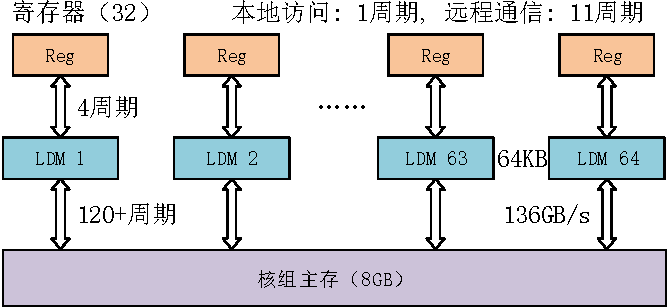
\includegraphics[width=.8\columnwidth]{memory_hieararchy-crop.pdf}
\caption{CPE的内存层次结构。顶层是高效的寄存器,访问或通讯需要花费1或11个周期;中间是大小为64KB的LDM高速缓存,访问LDM需要4个周期;底层是所有从核共享的8GB主存,访问需要120+个周期,带宽为136GB/s。}
\label{fig:sunway_mem}
\end{figure}

图~\ref {fig:sunway_mem}描述了申威26010处理器的内存层次结构和访问延迟。每个核组的内存总量为8GB,带宽为34 GB/s,由四核组组成的申威处理器共有32GB内存,内存峰值带宽为136GB/s。在从核阵列中,每个从核包含16KB指令缓存和64KB本地直接内存(local direct memory, LDM)。LDM高速缓存的带宽为与CPU中的L1缓存相当,但需要开发者针对不同应用进行精细的手动管理,这是应用优化的关键之一。此外,每个从核包含32个浮点寄存器与4个寄存器通信缓冲区。每个从核访问本地寄存器需要1个周期,若通过每一行或每一列的数据总线以及寄存器通信缓冲区进行寄存器通信则需要11个周期。良好的寄存器通信策略能有效地减少全局内存访问,节约DMA数据传输带宽和提高数据复用率。

% subsection 申威20610处理器概述 (end)

\subsection{并行计算模型} % (fold)
\label{sub:并行计算模型}

神威超算支持多种并行开发模型。不同的CPU和核组可采用消息传递接口(Message Passing Interface, MPI)组成多进程应用,一个CPU内的4核组也可使用著名的线程级并行计算模型——OpenMP模型。此外,神威超算还支持另外两种线程级并行模型,分别为OpenACC和Athread。这两种并行计算模型是针对神威超算异构众核结构开发的,也是最高效、最适合神威超算的编程模型。

申威处理器支持的OpenACC并行编程模型遵从OpenACC-2.0标准。OpenACC编程模型与OpenMP编程模型的用户体验类似,用户只需在核心循环代码块之前添加OpenACC制导语句,调用自动化并行编译工具编译后可生成从核并行代码。OpenACC编程模型显著地降低了并行程序的开发难度。除了申威处理器,NVIDIA公司也在大力推广OpenACC编程模型。对于NVIDIA公司而言,使用OpenACC编程的门槛、复杂度和用户代码量均远低于CUDA,因此更易于让科学计算从业者接受。OpenACC虽然降低了编程的门槛和复杂度,但却对编译器提出了更高的要求。OpenACC的性能一方面取决了用户是否正确使用OpenACC制导语句,更重要的是编译器能否将OpenACC制导语句和源代码最终翻译成高效的并行计算代码,并充分利用硬件的各种特性提升计算性能。目前申威26010处理器的OpenACC编程模型适用于简单的循环操作,在复杂的计算中无法发挥最优性能。

Athread并行模型通过使用Athread线程库手动编写从核代码的方式可以精细地控制每一个从核。申威处理器的OpenACC编译器也是将OpenACC代码转换为Athread代码,并调用从核编译器生成从核目标文件。因此用户可以首先使用OpenACC并行模型执行初步优化,然后调用OpenACC编译器生成Athread代码,再进行二次开发,这一定程度上能降低开发工作量。Athread线程库与Pthread线程库类似,支持对每个从核独立的计算、调度、同步等等操作。此外,Athread还支持申威26010处理器独有特性,如LDM高速缓存策略设计、从核间寄存器通信和向量化等等。复杂的核函数通常无法通过使用OpenACC并行模型来发挥极致性能,通常需要借助Athread线程库手动开发从核代码。

为了获得极致的计算性能,本研究使用Athread线程库精细地为每个从核划分任务,并在Athread线程库的基础上设计了一系列性能优化的方案,这将在后续的章节详细介绍。

% subsection 并行计算模型 (end)

\subsection{正演算法在申威处理器的计算挑战} % (fold)

神威·太湖之光在2016年的首次发布\citep{fu2016sunway},标志着世界最领先的超级计算机的运算能力首次超过了100Pflops,运算核心数量首次超过1000万。神威·太湖之光的计算能力也达到了前所未有的水平,其LINPACK性能相当于天河二号超级计算机的3倍,美国Titan超级计算机的5倍,然而内存系统却捉襟见肘。 如表\ref{tb:supercomputer-comp}所示,神威·太湖之光的总内存大小与其他系统相似(只比两个基于GPU的系统Piz Daint和Titan稍好),但字节浮点率却非常低,只有其他异构系统的五分之一,日本“京(K)"超级计算机的十分之一。 神威·太湖之光的计算和内存属性给科学应用的优化和扩展提出了严峻的挑战,特别是对于需要大内存空间和高内存带宽的地震模拟问题,打破内存的局限(内存墙)成为本研究最大的挑战。

\begin{table}[ht]
\footnotesize
\caption{神威·太湖之光超级计算机与其他领先超算系统的简要比较}
\label{tb:supercomputer-comp}
\center
\begin{tabular}{cccccc}
\hline
   & 峰值性能 & LINPACK性能 & 内存总量  &内存带宽 & 带宽/峰值性能 \\
   & (Pflops) & (Pflops) & (TB) & (TB/s) & (字节/Flop) \\
   \hline
   神威·太湖之光 & 125 & 93 & 1,310 & 4,473 & 0.038 \\
   天河二号 & 54.9 & 33.9 & 1,375 & 10,312 & 0.188 \\
   Piz Daint & 25.3 & 19.6 & 425.6 & 4,256 & 0.168 \\
   Titan & 27.1 & 17.6 & 710 & 5,475 & 0.202 \\
   Sequoia & 20.1 & 17.2 & 1,572 & 4,188 & 0.208 \\
   K & 11.28 & 10.51 & 1,410 & 5,640 & 0.5 \\
\hline
\end{tabular}
\end{table}

与神威超算的超大计算规模和强大计算能力相比,内存容量和内存带宽则是神威超算的一大不足。虽然每个节点只有32GB内存,但内存容量方面的不足可通过神威超算大量的节点和高效的网络通信将大规模算例扩展到更多的节点来弥补。然而在内存带宽方面,神威超算每个节点的内存带宽为136GB/s,仅为Intel KNL的1/3以及NVIDIA GPU的1/5,给许多访存受限问题提出了巨大的挑战。本文研究的正演算法的核心计算是显示时间的有限差分算法,计算模式为$Stencil$运算,这是典型的访存受限问题。在三维弹性波地震模拟中,每个核函数涵盖了20-50个三维数组,这进一步加剧了访存的挑战。

如第\ref{sub:神威超算软硬件环境}节所述,深度的从核优化需使用Athread并行模型,并合理利用LDM高速缓存。从核计算的基本流程为:(1)主存中的数据通过DMA方式传输LDM高速缓存;(2)从核从LDM高速缓存中取数据并执行相关运算;(3)通过DMA将运算结果从LDM传输到主存。

作为访存受限问题,$Stencil$计算的主要开销在于DMA传输,这由两方面因素决定:DMA数据传输总量和DMA传输带宽。在申威处理器中,每个核组有$8\times8$的从核阵列,每个从核都需要通过DMA将数据在主存和LDM中来回传输。与MPI通信类似,每个核组主存的划分方式、64个从核的逻辑排列方式都会对DMA数据传输总量造成影响。当数组的数量增大时,影响也随之增大。


虽然申威处理器每个核组的峰值内存带宽为34 GB/s,然而在实际应用中,大多数应用都无法达到峰值带宽。DMA传输带宽与DMA传输的连续数据块大小有密切的正相关关系(如表
\ref{tb:sw-bw}所示)。由表可见,当DMA连续传输块大小不足128字节时,DMA的传输带宽不足理论带宽的一半。只有当DMA连续传输块大小超过512字节时,才能达到较合理的内存带宽。

\begin{table}[thb]
\caption{单核组DMA连续传输块大小对应的实测带宽(GB/s)}
\label{tb:sw-bw}
\centering
\begin{tabular}{|c|c|c||c|c|c|}
  \hline
  块大小(字节) & $Get$ & $Put$ & 块大小(字节) & $Get$ & $Put$ \\
  \hline
  32&4.31&2.56& 512&27.42&30.34\\
  \hline
  64&9.00&9.20& 576&25.96&28.91\\
  \hline
  128&17.25&18.83& 640&29.05&32.00\\
  \hline
  192&17.94&19.82& 1024&29.79&33.44\\
  \hline
  256&22.44&25.80& 2048&31.32&35.19\\
  \hline
  384&22.88&24.67& 4096&32.05&36.01\\
  \hline
\end{tabular}
\end{table}

本文研究的三维弹性波地震模拟包含30-50个数组,所有的三维数组都需要频繁读写到LDM中,读写和划分的策略会直接影响DMA数据传输的总量。另一方面,由于数组总量多,使得每个数组在LDM中可容纳的元素少,导致DMA的连续数据块很小,这极大地制约着DMA的传输带宽。因此,$Stencil$运算在申威处理器中的性能优化主要集中在如何降低DMA数据传输总量和如何提升DMA传输带宽。

\section{最小DMA数据传输方案} % (fold)
\label{sec:最小DMA数据传输方案}

高效的从核计算所需的数据必须从LDM中获取而非直接从共享主存中读取。但每个从核中LDM的大小仅有64KB,在包含大量数组的核函数中,每个数组能够分配的LDM缓存空间非常有限。对于$Stencil$等访存受限问题,从核优化的重点在于如何缩短数据在主存和LDM中的传输时间。缩短DMA传输的时间有两个方法,减少数据传输总量和提升DMA传输带宽。本节讨论如何降低DMA数据传输总量。

\subsection{单从核数据传输方案推导}

在$Stencil$计算中,每更新一个中心点需要访问周围的其他格点。LDM空间有限,无法储存整个二维或者三维数组(波场),因此需要对波场进行划分。划分后的每个子波场包含中心区域和Halo区域。不同的划分会产生不同的Halo区域,从而影响DMA数据传输总量。本小节推导出在$Stencil$运算在二维划分下最小的DMA数据传输总量。

\begin{figure}[ht]
  \centering
  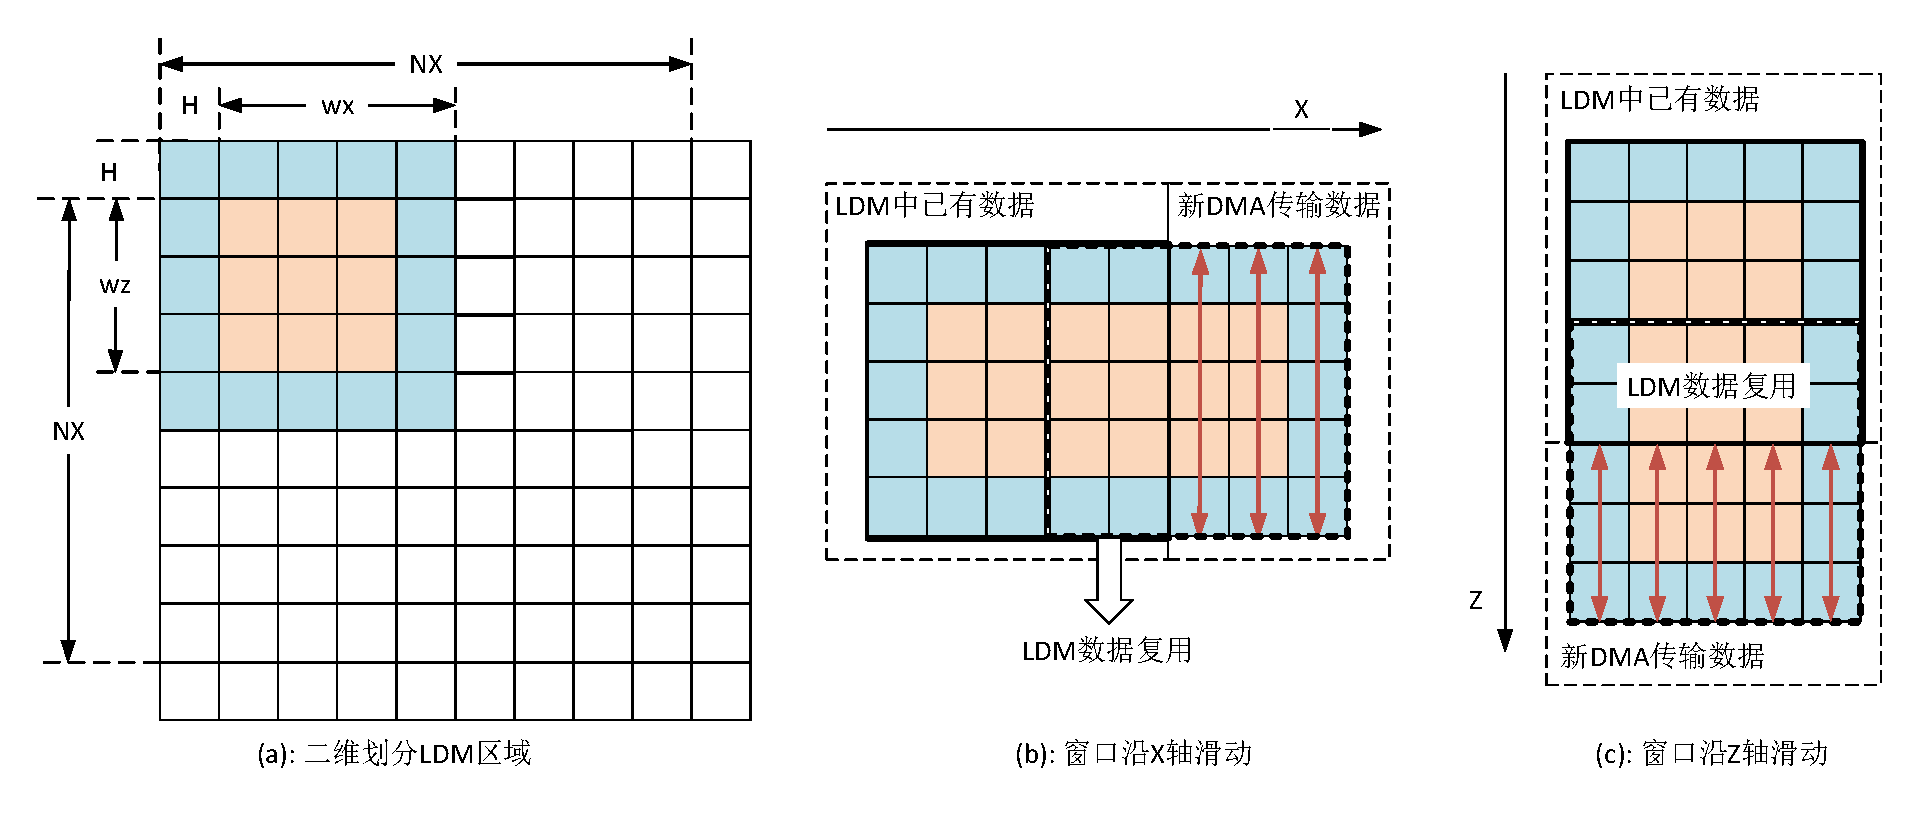
\includegraphics[width=1.0\columnwidth]{单从核2D划分最小DMA传输.pdf}
  \caption{单从核2D划分最小DMA传输。}
  \label{fig:cpe-2d-derive}
\end{figure}

如图\ref{fig:cpe-2d-derive}(a)所示,设数组的大小为$NZ\times NX$,其中Z轴是数组的快轴。Halo区域的宽度为$H$,每个数组在LDM所占的空间为$S=(wx+2H)\cdot(wz+2H)$,计算所需的格点都存储在这片空间中,称之为LDM窗口。窗口可以沿Z轴或者X轴滑动(如图\ref{fig:cpe-2d-derive}(b)(c)所示):
\begin{itemize}
  \item 当窗口沿着X轴滑动时,原窗口最右列的Halo区域能够被新窗口完全复用,新窗口只需读取右边四列数据。
  \item 当窗口沿着Z轴滑动时,原窗口最下行的Halo区域能够被新窗口完全复用,新窗口只需读取下面四行数据。
\end{itemize}

虽然两种滑动方式的DMA传输数据量相同,但效率却有差异。但由于数组的快轴是Z轴,沿着X轴滑动时,新窗口需调用4次DMA,每次DMA的大小为5个元素;而沿着Z轴滑动时,新窗口需调用5次DMA,每次DMA的大小为4个元素。由表\ref{tb:sw-bw}可知,DMA传输的连续数据块越大时能获得的带宽也越大,因此窗口沿着X轴从左向右滑动更有利于提高DMA传输效率。

公式\ref{eq:单从核二维划分最小DMA传输}描述二维划分下最小的DMA数据传输总量
\begin{equation}
  \min_{wx,wz} D(wx,wz) = (wz+2H)\cdot(NX+2H)\cdot\frac{NZ}{wz},
  \label{eq:单从核二维划分最小DMA传输}
\end{equation}
其中$(wz+2H)\cdot(NX+2H)$表示每次沿着X轴滑动所需传输的数据总量,$\frac{NZ}{wz}$表示再次从左至右滑动的次数。公式\ref{eq:单从核二维划分最小DMA传输}化简后可得公式\ref{eq:单从核二维划分最小DMA传输2}。
\begin{equation}
  \min_{wz} D_{1cpe}(wz) = (1+\frac{2H}{wz})\cdot(NX+2H)\cdot NZ,
  \label{eq:单从核二维划分最小DMA传输2}
\end{equation}

可以看到,$wz$与$D_{1cpe}(wz)$呈反相关,当$wz$越大时,$\frac{NZ}{wz}$越小,即再次从左至右滑动的次数越少,由于每次从左至右滑动时都需要额外读取上下边界的Halo区域,因此轮数越少,传输总量$D_{1cpe}(wz)$越小。

\subsection{64从核数据传输方案推导}
公式\ref{eq:单从核二维划分最小DMA传输2}描述的是一个从核执行DMA传输的最优情况。每个核组有64个从核,64个从核的不同排列和划分方式也会对DMA的数据传输总量造成影响。现推导单核组64从核同时进行计算和DMA传输时,最小的传输总量。

\begin{figure}[ht]
  \centering
  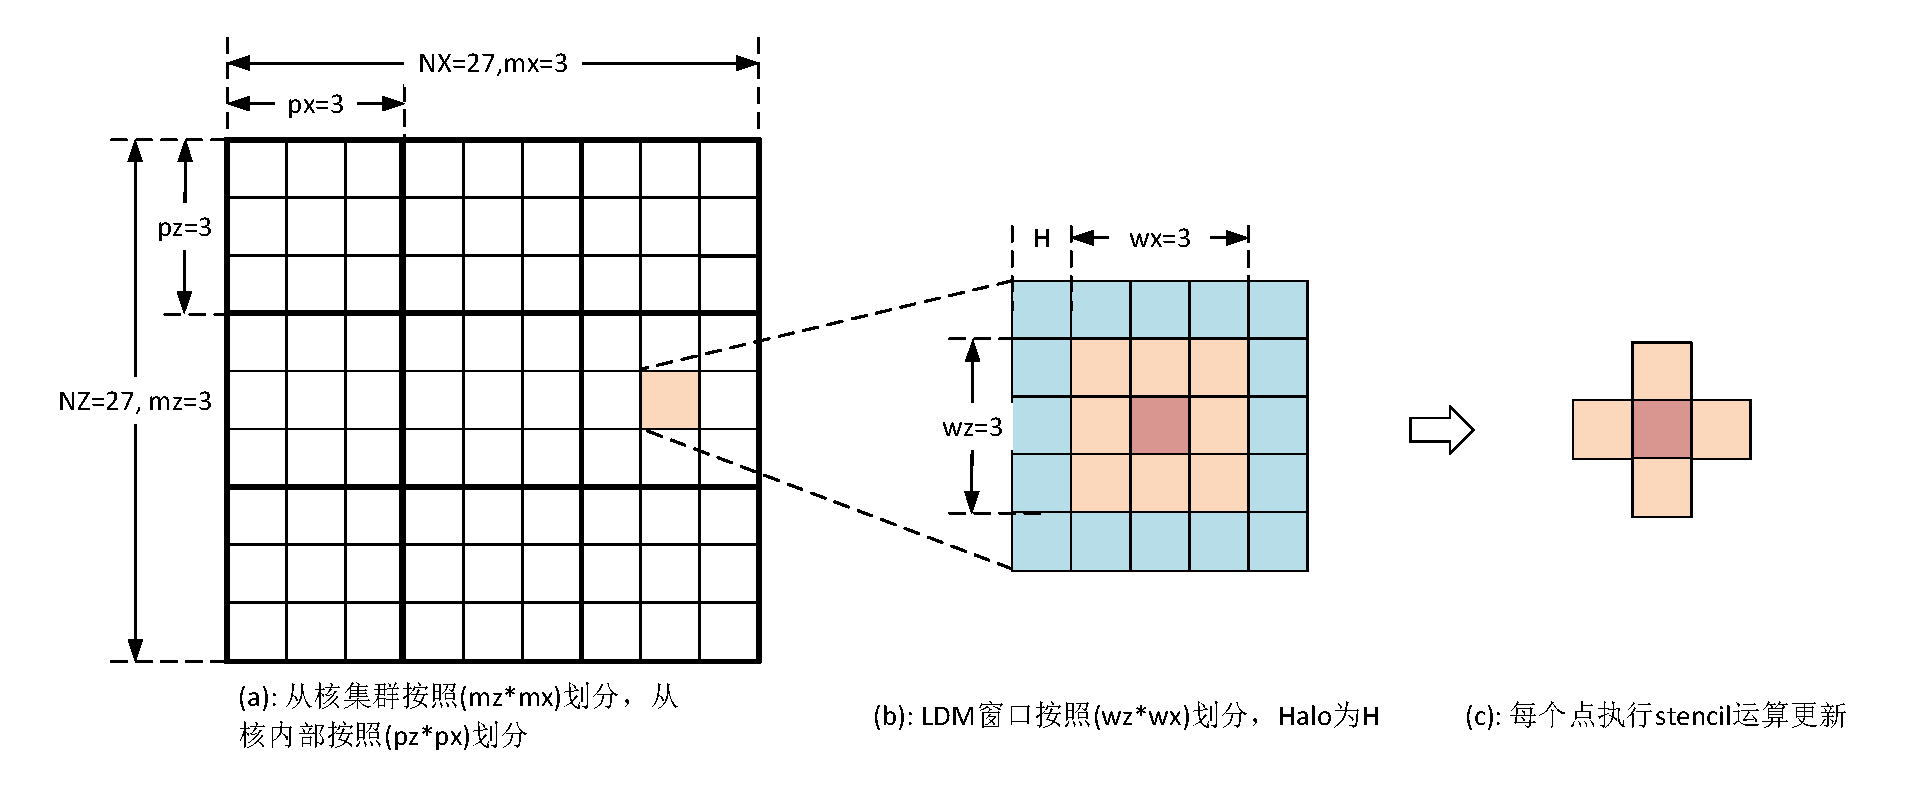
\includegraphics[width=1.0\columnwidth]{多从核2D划分最小DMA传输.pdf}
  \caption{多从核2D划分最小DMA传输。}
  \label{fig:multi-cpe-2d-derive}
\end{figure}

如图\ref{fig:multi-cpe-2d-derive}所示,设每个MPI进程需要更新的网格为$NZ\times NX$,每个核组的从核按照$mz \times mx$进行划分。每个从核计算的网格需要进一步划分才能放进64KB的LDM中,设每个从核内按照$pz\times px$划分,使得划分后的每一个小块能加载到LDM中,此时LDM窗口的大小为$(wz+2H)\times(wx+2H)$。本文需要推导出当$mz$、$mx$与最小DMA数据传输量的关系。此时,最小DMA数据传输的优化函数变为
\begin{equation}
  \min_{mx,mz,px,pz} D_{64cpe}(mx,mz,px,pz) = (\frac{NZ}{mz\cdot pz}+2H)\cdot(\frac{NX}{mx}+2H)\cdot pz,
  \label{eq:多从核二维划分最小DMA传输}
\end{equation}
化简可得
\begin{equation}
  \min_{mx,mz,pz} D_{64cpe}(mx,mz,pz) = (\frac{NZ}{mz}+2H\cdot pz)\cdot(\frac{NX}{mx}+2H),
  \label{eq:多从核二维划分最小DMA传2}
\end{equation}
且当64个从核都进行参与时,满足以下条件
\begin{equation*}
    \left\{\begin{matrix}
mx\times mz=64\\
1\le mz \le 64 \\
pz \ge 1 \\
1 \le \frac{NZ}{mz\cdot pz} \le Z_{max}
\end{matrix}\right.
\Leftrightarrow
  \left\{\begin{matrix}
mx\times mz=64\\
1\le mz \le 64 \\
1 \le pz \\
\frac{NZ}{mz\cdot Z_{max}} \le pz \le \frac{NZ}{mz}
\end{matrix}\right.。
\end{equation*}
其中,$Z_{max}$为每个从核LDM中最多可用来分配给Z轴的空间。将$mx=\frac{64}{mz}$代入到公式\ref{eq:多从核二维划分最小DMA传2}中可得
\begin{equation}
  \min_{mz,pz} D_{64cpe}(mz,pz) = \frac{NX\cdot NZ}{64}+\frac{NZ}{mz}\cdot 2H+\frac{NX\cdot mz \cdot pz}{64} \cdot 2H + pz\cdot 4H^2,
  \label{eq:多从核二维划分最小DMA传3}
\end{equation}

(1)若$pz \ge \frac{NZ}{mz\cdot Z_{max}} \ge 1$,代入公式\ref{eq:多从核二维划分最小DMA传3}可得
\begin{equation}
  \min_{mz} D_{64cpe}(mz) \ge \frac{NX\cdot NZ}{64}+\frac{NZ}{mz}\cdot 2H+\frac{NX\cdot NZ}{64\cdot Z_{max}} \cdot 2H + \frac{NZ}{mz\cdot Z_{max}}\cdot 4H^2,
  \label{eq:多从核二维划分最小DMA传4}
\end{equation}
则$D_{64cpe}(mz) $与$mz$呈反相关,当$mz$越大,$D_{64cpe}(mz) $越小。当$mz=64, mx=1, pz = \frac{NZ}{64\cdot Z_{max}}$时,$\min_{mz} D_{64cpe}(mz=64)$最小。

(2)若$\frac{NZ}{mz\cdot Z_{max}} < 1$,则$pz\ge 1$,代入公式\ref{eq:多从核二维划分最小DMA传3}可得
\begin{equation}
\begin{aligned}
  \min_{mz,pz} D_{64cpe}(mz,pz) &\ge \frac{NX\cdot NZ}{64}+\frac{NZ}{mz}\cdot 2H+\frac{NX\cdot mz}{64} \cdot 2H + 4H^2 \\
  &\ge \frac{NX\cdot NZ}{64}+2H\cdot2\sqrt{\frac{NZ}{mz}\cdot\frac{NX\cdot mz}{64} } + 4H^2 \\
  &=\frac{NX\cdot NZ}{64}+\frac{H}{2}\sqrt{NX\cdot NZ}+ 4H^2
  ,
\end{aligned}
  \label{eq:多从核二维划分最小DMA传5}
\end{equation}
当且仅当$\frac{NZ}{mz}=\frac{NX\cdot mz}{64}$时,等号成立。此时$mz=8\sqrt{\frac{NZ}{NX}}$,$mx=8\sqrt{\frac{NX}{NZ}}$。并可推出$\frac{mx}{mz}=\frac{NX}{NZ}$。此时$pz=1$。

通过公式\ref{eq:多从核二维划分最小DMA传4}可得,在充分利用所有从核进行二维划分的情况下,满足以下条件可使DMA的数据传输总量最小:
\begin{itemize}
  \item 当$pz \ge \frac{NZ}{mz\cdot Z_{max}} \ge 1$时,将64个从核按照$64\times 1$进行排布,可获得最小DMA数据传输总量;
  \item 当$\frac{NZ}{mz\cdot Z_{max}} < 1$时,从核按照$\frac{mx}{mz}=\frac{NX}{NZ},pz=1$进行排布,可获得最小DMA数据传输总量。
\end{itemize}

\subsection{基于寄存器通信的从核Halo更新}
\label{sub:寄存器通信}

推导出最小的DMA数据传输总量的前提是核组内的64个从核能够进行数据交互,且交互的成本很低甚至可以忽略不计。申威26010处理器与其他主流处理器相比,最与众不同的一个功能是核组内的CPE能进行寄存器通信。由64个CPE组成的从核阵列中共有8个列通信总线和8个行通信总线,这些总线成为了CPE之间进行快速寄存器通信的通道,为不同的CPE提供了高速的数据共享能力。寄存器通信是提升$Stencil$计算数据重用率的重要方法。

使用了基于寄存器通信的Halo交换后(如图\ref{fig:64by1-reg}所示),每个CG内部的CPE线程只需要加载其相应的中心计算区域,并且可以通过寄存器通信方案从相邻线程获取所需的Halo区域。核组内的Halo区域交换可通过寄存器通信完成,但核组间的Halo区域交换仍需要通过共享主存来完成。

寄存器通信是通过行、列通信总线中的一对\emph{Put}和\emph{Get}API接口来实现的。发送方CPE使用\emph {Put}接口将256位寄存器数据发送到接收方CPE的寄存器通信缓冲区,然后接收方CPE使用\emph{Get}操作将256位数据从寄存器通信缓冲区中取回本地通用寄存器中。

寄存器是从核中非常稀有且宝贵的资源。每个从核只有8个256位的寄存器可用于通信。寄存器的发送和接受是同步操作,批量发送把接收方缓冲区填满,阻塞发送方线程的正常执行。不当的寄存器通信操作反而会降低计算性能,甚至会造成不同从核线程死锁。本文设计了间隔收发同步通信策略实现寄存器高效通信,通信的步骤如下:
\begin{itemize}
  \item 编号为奇数的从核统一执行寄存器发送操作,将1个256位的向量发送给编号为偶数的从核寄存器缓冲区;
  \item 同时,编号为偶数的从核执行寄存器接收操作,等待其他寄存器向其发送数据;
  \item 奇数寄存器发送、偶数寄存器接收完毕之后,以同样的策略执行偶数寄存器发送、奇数寄存器接收操作;
  \item 以同样的方式通信下一个256位向量。
\end{itemize}

\begin{figure}[ht]
\centering
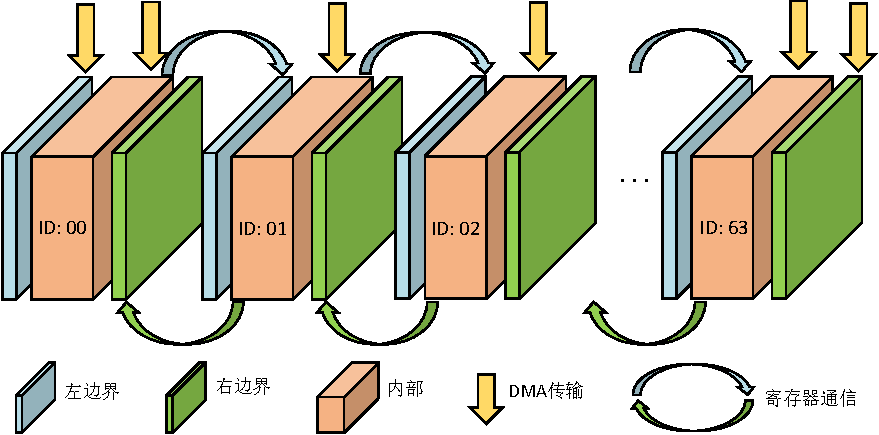
\includegraphics[width=0.7\columnwidth]{寄存器通信-crop.pdf}
\caption{同一核组内的64个CPE使用寄存器通信。}
\label{fig:64by1-reg}
\end{figure}

由于用于通信的总线只能连接同一行或者同一列的从核,只有在同一行或者同一列的CPE才能够进行寄存器通信。如果两个CPE分布在不同的行和不同的列中,则需要通过中转,使用多次寄存器通信来实现数据交换。

正如在第\ref{sec:最小DMA数据传输方案}节中的推导,在大多数情况下可采用$ 64 \times1 $的CPE线程配置。在这样的配置中,需要交换数据的多数的CPE线程将不在同一行或列中。为了解决这个问题,并尽可能减少所需的寄存器通信操作次数,本文设计了一个特定的CPE ID重新映射方案。

如图~\ref{fig:id-remapping}所示,对于奇数行,逻辑 CPE ID(括号内的ID)在映射后保持与原始硬件CPE ID相同(ID外部的ID括号);对于偶数行,逻辑 CPE ID在映射后则与原始硬件CPE ID相反。从核ID重新映射之后,可以保证需要寄存器通信的从核位于同一行或同一列中,也可快速索引到目标从核线程号。

\begin{figure}[ht]
\centering
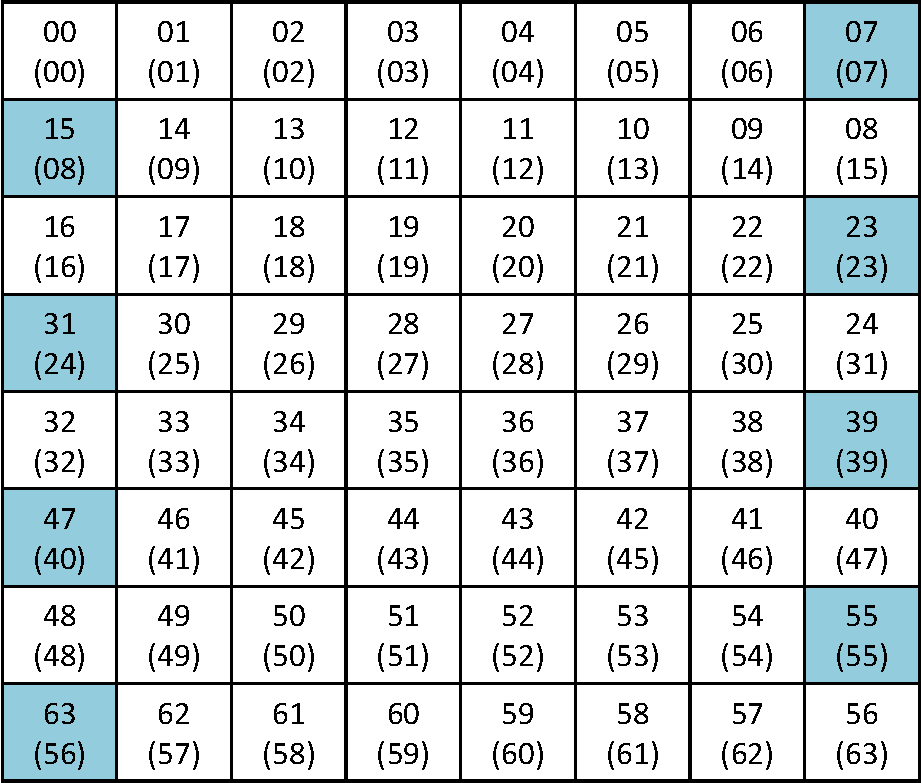
\includegraphics[width=0.5\columnwidth]{从核ID重映射-crop.pdf}
\caption{
从核ID重新映射方案确保了所有相邻CPE线程间的寄存器通信操作。括号外的ID为原始硬件从核ID,括号内的ID是重新映射的逻辑从核ID。}
\label{fig:id-remapping}
\end{figure}

\section{增大DMA数据传输带宽方案} % (fold)

最小DMA数据传输方法侧重降低DMA数据传输总量,本节提出增大DMA数据传输带宽的两种方案——共位数组融合和数据布局转换。

\subsection{共位数组融合}
\subsubsection{朴素共位数组融合}

第\ref{sec:最小DMA数据传输方案}节介绍了最小DMA数据传输和寄存器通信方案。然而,即便采用上述的最佳并行方案,在只有64KB的LDM中,由于三维弹性波正演方法包含大量数组,能够分配给每个数组的缓存空间非常有限的。

三维$Stencil$运算需访问当前元素的上下左右前后六个方向的不同格点,因此需要将三维子区域载入LDM中。三维区域在内存中只有一个维度是连续,DMA只能按照连续的内存进行多次数据传输。DMA传输的启动开销虽然不大,但DMA传输的带宽受连续传输数据块大小的严重影响。

例如,地震波正演的速度更新核函数需要读取10个不同的三维数组:$ u $,$ v $,$ w $,$ xx $,$ yy $,$ zz $,$ xy $,$ xz $,$ yz $,$ d $,分别是速度的三个分量、应力的六个分量以及密度。根据第\ref{sec:最小DMA数据传输方案}节的推导可得
\begin{equation}
\begin{aligned}
C_z &\cdot C_y = 64  \\
W_z \cdot W_y \cdot W_x \cdot N_{array} &\cdot N_{bytes\_per\_variable} < 64 \times 1024
\end{aligned}
\label{eq:wzy}
\end{equation}
其中$ N_{array} $表示当前计算函数所需的3D数组的数量,$N_{bytes\_per\_variable}$表示每个变量的字节数。为了完成空间四阶精度的中心差分运算,LDM缓存中至少需要沿着$x$方向加载五个平面(以第三个平面为中心,前后两个面各为差分长度),因此$ W_x $的最小值为5。$(W_y-2H)$为加载到LDM中的有效区域,至少需要将$ W_y $设置为9(对于$ H = 2 $)以保持Halo成本处于合理的水平。
因此,在10个输入数组的情况下可以从公式\ref{eq:wzy}推导出:
\begin{equation}
W_z \cdot 9 \cdot 5 \cdot 10 \cdot 4 < 64 \times 1024\\
\label{eq:wzy1}
\end{equation}
可得$ W_z $的最大值为32。在这种情况下DMA传输的连续块的大小为128字节。由表\ref{tb:sw-bw}可知对应的带宽约为17GB/s,仅为内存峰值带宽的50\%,利用率较低。

三维弹性波正演中DMA批量传输数据少的现象在二维或声波方程中并不明显。在二维声波方程中不需要考虑应力和空间分量,程序中数组的总量约为三维弹性波情景中的20\%甚至更低,这使得二维声波方程中每个数组可利用的LDM空间是三维弹性波中的5倍,DMA批量传输数据块也随着增大。不过二维声波方程扩展到三维弹性波方程过程中虽然数组总量增大了,但变量的物理含义变动较小:增加了应力变量、速度由原来的二维扩展到三维。这启发了本文作者提出共位数组融合方法。

%%%%%%%%%%%%%5看到这里%%%%%%%%%%%
仍以速度更新核函数为例,虽然该函数涉及到10个三维数组,但这10个数组可分成3组,分别代表速度(3个分量)、应力(6个分量)和密度。三个速度分量是彼此对称的,所执行的计算操作类似,六个应力分量也是如此。本研究称这三个速度分量($ u $,$ v $,$ w $)或这六个应力分量($ xx $,$ yy $,$ zz $,$ xy $,$ xz $和 $ yz $)为共位数组(co-located array),共位数组融合则分别将三个速度分量或六个应力分量融合成一个大数组。共位数组融合的过程如图\ref{fig:naive-fusion}所示。

\begin{figure}[ht]
\centering
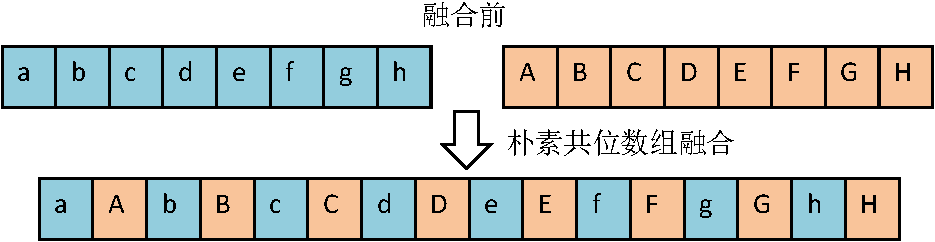
\includegraphics[width=0.9\columnwidth,page=1]{分块共位数组融合-crop.pdf}
\caption{朴素共位数组融合示例。}
\label{fig:naive-fusion}
\end{figure}

共位数组融合之后,从等式\ref{eq:wzy}中可以看到,只有三个单独的数组可以读取,则有
\begin{equation}
W_z \cdot 9 \cdot 5 \cdot 3 \cdot 4 < 64 \times 1024\\
\label{eq:wzy2}
\end{equation}
可得$ W_z $的最大值约为108。此时,DMA传输连续数据块大小为432字节,内存带宽利用率可提高到80%左右。 

在地震波正演的应力更新核函数,共位数组融合技术可以将DMA连续数据块从84字节增加到512字节,从而将有效内存带宽从50.47 GB/s提高到104.82 GB/s。

共位数组融合方法显著地提升了DMA传输带宽,但这种数组融合方法还面临着一个问题:无法向量化。本文称之为朴素共位数组融合方法。朴素共位数组融合方法可以将任意数量的数组进行融合,但由于不同数组的元素相互交错排列而无法实现向量化。虽然向量化无法显著提升$Stencil$等内存受限运算的性能,但能显著提升计算受限问题(如矩阵运算、卷积运算)的效率。本研究在朴素共位数组融合的基础上提出分块共位数组融合方法,使之支持向量化。

\subsubsection{分块共位数组融合}

申威26010处理器支持位宽为256比特的向量化操作,等价于支持4个连续double类型元素的算术运算。申威处理器建造之初为了更好的支持双精度浮点数的科学运算,向量化操作并不区分双精度和单精度浮点数,因此尽管单精度浮点数的位宽只有双精度浮点数的一半,申威处理器也支持4个连续float类型元素的向量化运算。分块共位数组融合策略把4个连续的元素合成一个单元块,然后使用朴素共位数组融合,融合过程如图\ref{fig:block-fusion}所示。

\begin{figure}[ht]
\centering
\includegraphics[width=0.9\columnwidth,page=2]{分块共位数组融合-crop.pdf}
\caption{分块共位数组融合示例。}
\label{fig:block-fusion}
\end{figure}

不管需要融合的数组数量为多少,始终以同一个数组的4个元素为一块,保证向量化的正常运算。

\subsection{数据布局转换} % (fold)
\label{sub:数据布局转换}

共位数组融合方案能有效增大DMA数据传输块大小,但只适用于能够进行融合的数组,如速度的三个分量、应力的六个分量以及其他具有相同读写模式的变量。然而在完整的大地震模拟程序中,并非所有变量都能参与融合。对于不能进行数组融合的变量,DMA数据传输仍旧面临着传输数据块小的困境。本小节针对个别无法参与共位数组融合的变量提出另外一种增大DMA数据传输块大小的方法——数据布局转换法。

数据布局转换方法根据特定的从核划分方案对数组进行预处理,重排数组中的所有元素,使之在从核读写时能够增大DMA数据传输块大小。数据布局转换的基本思想如图\ref{fig:layout-trans}所示。在原始的并行策略中,每个从核需要读写对应的分块(如图\ref{fig:layout-trans}(b))所示,由于原始数据在内存中的排列仅沿着一个维度连续,每个从核仅能通过多次的小块读取来加载从核所需的2D平面,但每次DMA传输的连续数据块小,DMA性能低下。

为了保证每个从核所需的2D平面数据在内存中的连续性,每个从核在初始化阶段首先对自己需要处理的2D平面数据进行布局转换,转换后的结果如图\ref{fig:layout-trans}(b)所示,转换过程如下:

\begin{itemize}
  \item 主核为需要执行数据布局转换的数组新开辟空间。由于每个从核需要执行$Stencil$运算,新开辟的空间能够容纳$Stencil$运算中的Halo部分;
  \item 需要处理完整数据边界的从核从主存中读取边界,Halo区域在通过寄存器通信方式从邻居从核中获得;
  \item 从核处理的中心区域部分则按照图\ref{fig:layout-trans}(c)所示的地址变换算法计算新的地址。
\end{itemize}   

数据布局转换后,从核DMA数据传输块的大小从原来的$wz$变为$wz\times wy$,通常情况能够获得很好的DMA带宽。

\begin{figure}[ht]
\centering
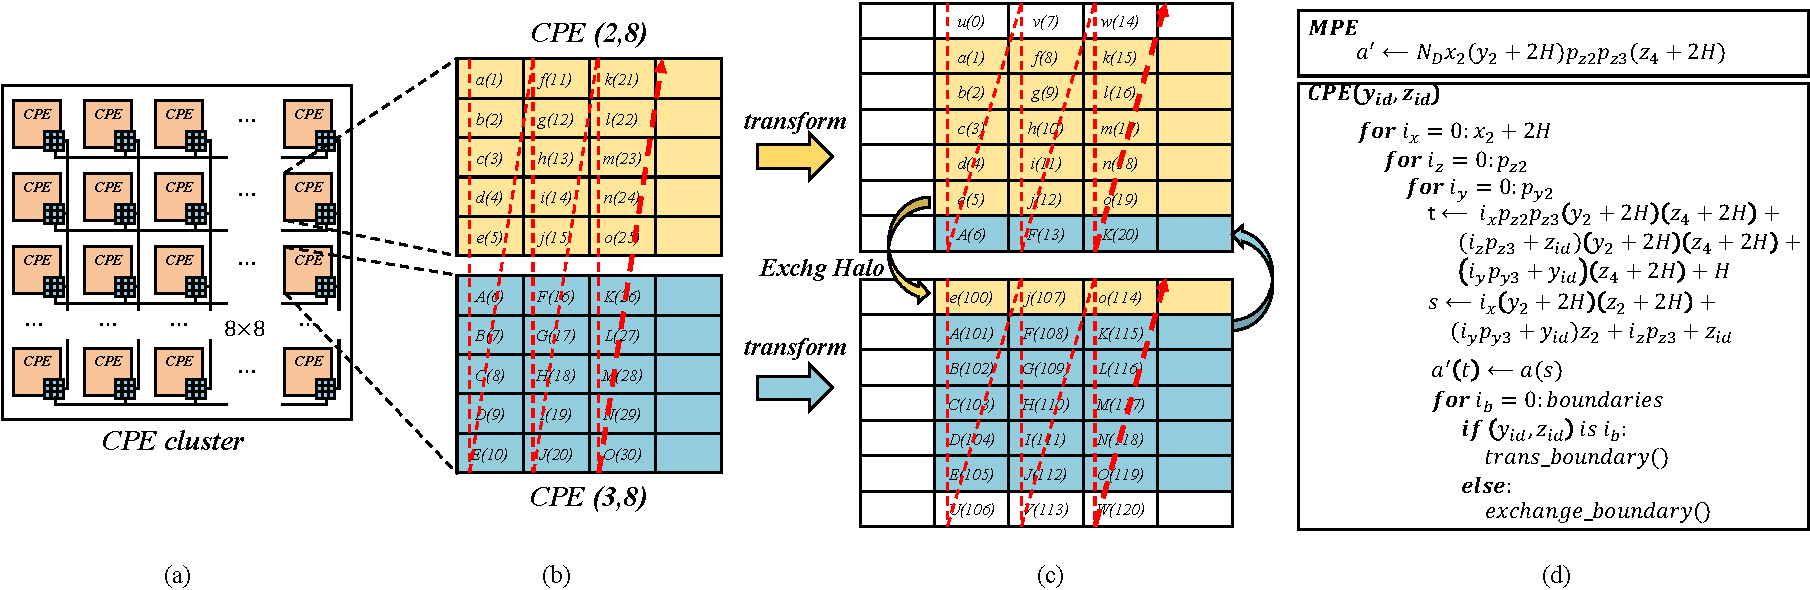
\includegraphics[width=1\columnwidth,page=1]{datalayouttransform-crop.pdf}
\caption{数据布局转换示例。}
\label{fig:layout-trans}
\end{figure}

数据布局转换方法虽能有效地针对无法参与共位数组融合的变量提升DMA带宽,然而如果该数组在每次计算更新后需要与邻近进程交换边界,数据布局转换则会打乱原来需要进行通信的元素位置。原来位于边界的元素执行地址转换之后可能位于三维数组中的任意位置,边界通信时无法按照规则的索引方式定位这些元素,只能通过地址逆转换还原数据布局,而这将进入额外的计算和访存开销。因此本文并不建议在需要与邻居进程通信的变量中使用数据布局转换策略。在真实的地震模拟中,只有速度和应力物理量需要执行MPI通信,他们可以使用共位数组融合方法。无法使用共位数组融合的物理量通常为介质参数如密度($\rho$),它们在整个程序中始终为常量,数据布局转换策略正好为这些数据提供了很好的增大DMA数据传输带宽的解决方案。

\subsection{内存对齐}

内存对齐是另外一种提升DMA数据传输效率的方法。DMA数据传输每次按128字节读取数据,未按照128字节对齐分配的数组在DMA数据传输时会降低DMA传输效率。例如,若DMA连续数据传输的大小为256字节,若主存中的数据未按照128字节对齐,则需要发起3次DMA传输,共传输384字节,其中有效数据为256字节。若主存中数据按照128字节对齐,则只需要发起2次DMA传输,效率为前者的1.5倍。

上文介绍的共位数组融合和数据布局转换方法并未考虑内存对齐,本小节讨论每一种方法的内存对齐。对于$Stencil$运算,从核的DMA数据传输可分为两部分,Halo区域和中心区域。朴素共位数组融合的数组数量不确定,因此只能在数组起始地址按128字节对齐,每个从核的计算起始地址和边界从核的Halo起始地址无法保证按128字节对齐。只有一个从核(第0号从核)能获得字节对齐带来的带宽收益。

分块数组融合按照向量化的要求保证每个数组有4个元素连续排列。地震模拟应用中数据类型通常使用单精度浮点数($float$),每个数组连续的字节数为16。如果正好有8个数组需要融合,则正好可实现128字节的内存对齐,然而实际情况并无法保证每次分块数组融合正好是8个数组。对于此类情况有两种对齐方式:Halo起始地址对齐和计算中心起始地址对齐,任意一种方式都容易实现,但只能获得其中一项带宽收益。本文研究Halo地址地址和中心计算起始地址同时对齐的方法:
\begin{itemize}
  \item Halo区域的起始地址对齐要求可以通过分配内存时按128字节对齐分配内存。
  \item 计算中心区域起始位置取决于Halo区域的长度,Halo区域的长度取决了差分算子长度和融合的数组数量。如果Halo区域的字节长度不能整除128,则计算中心区域的起始地址无法按照128字节对齐。这种情况下可通过扩展Halo区域长度,使之能被128整除。
  \item 尾部区域也采用同样的方式进行区域扩展,保证所有从核读取的Halo区域和计算中心区域也按照128字节对齐。
\end{itemize}

数据布局转换不涉及多个数组合并,因此内存对齐较为简单。首先在内存分配时保证按128字节对齐,然后调整每个从核的划分,使得每个从核读取的起始地址也按128字节对齐。

%数据布局转换的过程如图1所示,首先MPE开一个空间,之后CPE先进行中间区域的地址转换,之后判断是否为某一个边界,如果为边界则需要单独读取边界,如果不是边界则需要和邻居CPE交换边界来完成转换。而地址转换的地址转换为:首先,将整个z轴在原数组按照z4进行分层,而新数组则以z4+2H分层,但层数保持不变,旧的数组z轴长度为p_{z2}p_{z3}z_4也,即z_2,而新的数组z轴长度为p_{z2}p_{z3}(z4+2H),而y轴长度保持不变。因为我们是按照一个平面一个平面地转换,因此先计算x方向的偏移量,新数组为i_{x}p_{z2}p_{z3}(y_2+2H)(z_4+2H)。在新的数组中,数据在一个层中排列完之后再排列下一层,层的序号为(i_z p_{z3} + z_{id}),再乘以y轴长度y2+2H则为该层之前的偏移。之后在该层内部先计算y轴偏移(i_y p_{y3}+y_{id})(z_4+2H),之后再加上z轴上边界H偏移,即为该区域需要转换的首地址,而旧数组地址的计算为常规计算。之后通过拷贝操作来将旧数组拷贝到新数组。

% subsection 数据布局转换 (end)

% section 数据结构变换 (end)

\section{实时压缩/解压缩设计方案}
\label{sec:实时压缩/解压缩设计方案}
\subsection{实时压缩必要性分析与设计思路}

神威·太湖之光超级计算机作为目前世界最快的超级计算机,系统的内存上限为1PB。有限的内存容量限制了神威超算能够支持地震模拟的最大问题规模和分辨率。例如,唐山大地震模拟在模拟范围为320km $\times$ 320km $\times$ 40km的情况下能选择的分辨率最高为10m。这已经是同等计算区域下最高精度的模拟。如果想支持更高分辨率的地震模拟,即便是世界最快的神威超算也无能为力。

此外,地震模拟的核心数值算法是有限差分运算,有限差分运算的效率受限于神威超算的内存带宽的不足。神威超算的最大优势是高速的浮点运算,但有限差分算法却无法将浮点运算单元充分利用。访存受限的数值算法和神威超算较低的字节浮点率形成尖锐的矛盾。

本文基于神威超算的特殊体系结构提出实时压缩/解压缩设计方案,旨在解决上述挑战。压缩方案通过将程序内部变量和外部数据进行压缩,降低了神威主存和文件系统的容量开销,使得相同物理内存能够支持更大规模算例。另一方面,神威特殊的主从核结构、编程可控的LDM高速缓存使得压缩数据可在从核中进行解压和浮点运算。由于压缩后的数据量变小,数据通过DMA从主存传输到从核LDM的总时间也随之缩短,而压缩/解压引入的额外计算也让闲置的从核计算单元得以利用,因此较为理想地解决了上述第二个挑战。

图\ref{fig:compression-workflow}描述了主从核协同压缩方案计算流程。首先将外部输入数据(如震源、模型)压缩后存储在硬盘中,地震模拟程序将压缩后的数据去读到主存中,从核通过$dma\_get$等接口将数据从主存传输到从核LDM中,此时数据仍处于压缩状态;从核在LDM中对数据进行解压还原成标准的单精度浮点数,并使用浮点运算单元完成$Stencil$运算;计算完毕后再压缩结果数据,并通过$dmg\_put$接口将结果传回主存。

\begin{figure}[ht]
\centering
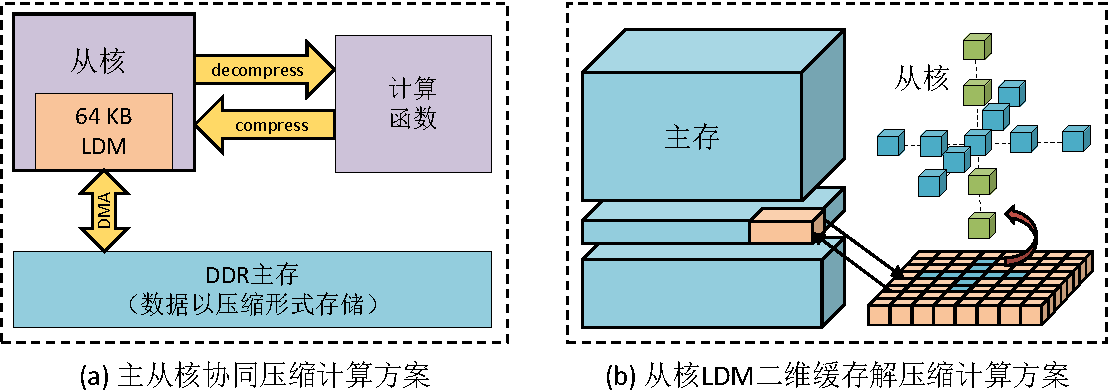
\includegraphics[width=0.9\columnwidth]{主从核协同压缩方案-crop.pdf}
\caption{主从核协同压缩方案计算流程。}
\label{fig:compression-workflow}
\end{figure}

\subsection{单精度浮点数压缩算法}

压缩方案的本质是以计算时间换取内存/存储空间,势必引入额外的计算开销。大地震模拟本是计算量大、耗时长的科学应用,如果压缩方案引入的额外计算开销太高,即便能够模拟更大规模的地震算例,也不具备现实意义。因此,高效的压缩算法是也压缩方案设计中一大重要环节。

传统的压缩算法如行程长度压缩算法(Run Length Encoding, RLE)、哈夫曼编码、Lempel-Ziv等对字节流进行压缩。这并不适合有限差分运算模式。例如四阶中心差分运算需要获取中心格点以及周围的各两个格点,这些格点在内存中是不连续的,几乎无法从压缩后的数据中索引差分计算所需的格点。因此,本文根据有限差分运算的计算模式定制了特殊的压缩算法。

设计压缩方案的另外一个考量是选择无损压缩或是有损压缩。无损压缩能够保持计算精度但需要较大的计算量且压缩率较低,而无损压缩在牺牲适量精度的情况下获得了较低的计算开销和较高的压缩率。地震模拟的数据通常用32位单精度浮点数表示,结果以地震波快照的形式呈现,因此对数据的精度有较高的容忍度。为了提高计算效率,本文提出并采用三种有损压缩算法,在可接受精度的前提下将32位浮点数压缩成16位浮点数。

\subsubsection{IEEE 754标准半精度浮点数压缩方法}
第一种压缩方法将IEEE 754单精度浮点数压缩成IEEE 754半精度浮点数。单精度浮点数的符号位、指数位和尾数位分别有1、8、23位,半精度浮点数的符号位、指数位和尾数位分别为1、5、10位(如图\ref{fig:ieeefloathalf}所示)。IEEE标准单精度浮点数与半精度浮点数之间的转换已有大量成熟工作\cite{van2008fast},本文工作将Scipy\cite{jones2014scipy}中的单精度-半精度浮点数转换开源代码移植到神威从核。

\begin{figure}[ht]
\centering
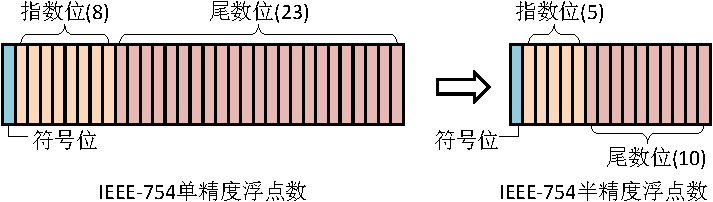
\includegraphics[width=0.8\columnwidth,page=1]{压缩浮点数表示形式-crop.pdf}
\caption{IEEE标准单精度-半精度浮点数表示方式。}
\label{fig:ieeefloathalf}
\end{figure}

在不考虑上溢(overflow)、下溢(underflow)、非规范化(denormalized)数的情况下,标准单精度-半精度浮点数转换核心算法如算法\ref{alg:ieeefloat}所示。
\begin{algorithm}[ht]
%\scriptsize
%\footnotesize
\small
\caption{IEEE标准单精度-半精度浮点数转换核心}\label{alg:ieeefloat}
\begin{algorithmic}[1]
\State \textbf{// 16位半精度转32位单精度}
\State uint32\_t \textbf{float16\_to\_float32}(uint16\_t h) \{
\State \quad\quad return ((h\&0x8000)<<16) | (((h\&0x7c00)+0x1C000)<<13) | ((h\&0x03FF)<<13);
\State \}
\State
\State \textbf{// 32位单精度转16位半精度}
\State uint16\_t \textbf{float32\_to\_float16}(uint32\_t f) \{
\State \quad\quad uint32\_t x = *((uint32\_t*)\&f);
\State \quad\quad return ((x>>16)\&0x8000)|((((x\&0x7f800000)-0x38000000)>>13)\&0x7c00)|((x>>13)\&0x03ff);
\State \}
\end{algorithmic}
\end{algorithm}

\subsubsection{动态指数位压缩方法}
IEEE单精度-半精度的转换算法简明高效,但由于半精度浮点数使用固定的指数位和尾数位,对于指数范围大于五位的浮点数,压缩方案会产生数值问题。另一方面,对于指数范围较小的变量,固定的五位指数位则变成了浪费。

\begin{figure}[ht]
\centering
\includegraphics[width=0.8\columnwidth,page=2]{压缩浮点数表示形式-crop.pdf}
\caption{动态指数位浮点数表示形式。}
\label{fig:ieeefloatdynamic}
\end{figure}

为了解决上述问题,本人工作提出了动态指数位压缩方法(如图\ref{fig:ieeefloatdynamic}所示)。这个压缩方法中的指数位和尾数位是动态确定的,不同的数组会得到不同的结果。指数位和尾数位的计算方法如公式\ref{eq:floatdynamic}所示:
\begin{equation}
  \begin{aligned}
    N_e &= \log(E_{max} - E_{min}) \\
    N_f &= 15 - N_e
  \end{aligned}
  \label{eq:floatdynamic}
\end{equation}
其中$N_e$表示指数位,$N_f$表示尾数位,$E_{max}$和$E_{min}$分别表示被压缩数组中元素最大的指数位数和最小的指数位数。

本方法最多可用15位表示指数(实际情况不会出现15位指数),远大于标准单精度浮点数的8位,足以保证全动态范围覆盖。对于指数范围较小数据,本方法则可为尾数部分保留更多表示位数,提高压缩后数据的精度。但是,由于涉及对数或除法运算,本方法唯一的缺点是计算成本相对较高。

\subsubsection{浮点数归一化压缩方法}
在IEEE标准的单精度浮点数表示中,大部分为归一化数(normalized value)。令符号位、指数位、尾数位分别为$S$、$E$和$F$,则归一化浮点数的数值为
\begin{equation}
  f(S,F,E) = (-1)^S \cdot 1.F^{E-127}
\label{eq:floatrepresent}
\end{equation}

浮点数归一化压缩方法对浮点数进行归一化,将同一数组的所有值归一化到1到2之间的范围(如公式\ref{eq:floatnormalized}所示),根据归一化浮点数的表示方法(公式\ref{eq:floatrepresent})可知,该浮点数的指数位$E$恒等于127。
\begin{equation}
\begin{aligned}
  v_{normalized} &= \frac{v - v_{min}}{v_{max} - v_{min}} \\
  v_{compressed} &= (v_{normalized} << 9) >> 7
\end{aligned}
\label{eq:floatnormalized}
\end{equation}

对范围为(1,2)的浮点数进行压缩,由于指数位恒等于127,压缩时无需对指数位进行存储,只需保留符号位和尾数位即可。公式\ref{eq:floatnormalized}中将归一化后的浮点数左移9位,然后右移7位得到16位数,即为压缩后的结果(如图所示\ref{fig:ieeefloatnormalized})。值得注意的是,在左移的过程中,符号位消失,因此需要在左移之前将符号位保存在第16位尾数中。

\begin{figure}[ht]
\centering
\includegraphics[width=0.8\columnwidth,page=3]{压缩浮点数表示形式-crop.pdf}
\caption{归一化浮点数表示形式。}
\label{fig:ieeefloatnormalized}
\end{figure}

上述展示的三种压缩方法仅针对地震模拟处理了大部分常规浮点数,并未覆盖浮点数的全部范围,如$NaN$,$INF$等等,这些数值并未在地震模拟应用中出现。

\subsection{压缩算法性能与精度分析}

压缩方案本身会引入额外的计算(主要是整数运算)以及密集的内存和高速缓存访问。即使所有的压缩/解压缩操作都发生在LDM中,频繁的LDM读写也会严重降低CPE的计算效率。因此,本文工作的第一个压缩版本只能达到不压缩版本的1/3性能。为了降低压缩方案的性能损失,本文进行了一系列优化:

\begin{itemize}
  \item 根据不同的物理量对精度敏感度不同,在满足精度要求的情况下,选择计算复杂度较低的算法;
  \item 在从核LDM中对压缩数据执行分块解压缩,以降低减少重复解压次数和LDM读写次数。
  \item 将解压缩和计算代码紧密地(在汇编代码级别)耦合以最大化寄存器中的变量的寿命,减少对LDM的读写次数;
\end{itemize}

将压缩方案与地震波传播相结合并经过深度优化后可获得24\%的计算性能提升,因为压缩方案可以在相同的物理带宽情况下处理更多的数据。换而言之,对于有限差分这类访存受限问题,压缩方案使得需要处理的数据总量降为原来的一半,极大地缩短了DMA数据传输时间。另一方面,在压缩率为50\%(32位浮点数压缩为16位数)的情况下,神威超算上可解决的最大问题规模扩大了一倍。这是一种通过软件形式突破硬件内存限制的方法。

实时压缩算法的精度对地震模拟有至关重要的影响,本研究通过理论和实践分析每个变量的精度敏感性,为其定制合适的压缩算法。经过精细的调优操作为不同变量选取了可接受精度范围内性能最好的压缩算法。压缩算法的精度算例分析将在唐山大地震算例中详细描述。

\section{本章小结}

本章研究在体系结构层面提出了面向申威异构众核处理器的地震正演并行优化方法,分别从降低内存传输总量和提升内存传输带宽两方面打破申威处理器的内存墙。本章首先推导出最小DMA数据传输方案以完成有限差分运算,并借助从核寄存器通信特性更新有限差分边界。在增大DMA数据传输带宽方面,本章提出了共位数组融合和数据布局转换两种方法对底层数据结构进行改动,能够显著提升DMA数据传输带宽。在内存容量达到极限的情况下,本章提出了实时压缩/解压缩方案对模拟变量进行压缩,在可接受的精度损失情况下能支持更大规模的地震模拟,将应用程序的可用内存大小和带宽提升到全新的高度。

% 流水线指令重排优化

% chapter 面向申威26010异构众核架构的并行优化方法 (end)